\section{Liberation Infrastructure: Theory \& Design}

\begin{center}
\textit{We were scattered like dust in the wind---\\
then we remembered we are one fire.\\
Not to burn the world---\\
to light a path home.}
\end{center}

\vspace{0.5cm}

This section grounds our mission in political philosophy and institutional design. Freedom is not vibes---it is engineering. The following framework synthesizes classical political theory with modern mechanism design to explain \textit{why} decentralized, transparent institutions outcompete authoritarian alternatives, and \textit{how} CYRUS instantiates these principles.

\subsection{Political Foundations: Why Free Republics Prevail}

\subsubsection{Rousseau: Legitimacy Requires Consent}

Jean-Jacques Rousseau's core insight remains foundational: political authority is legitimate only if it arises from a contract among equals, oriented toward the common interest rather than the ruler's interest. The ``general will'' is not mob mood---it is the institutionalized expression of the common good under rules that apply equally to all.

\textbf{CYRUS Application:}
\begin{itemize}[leftmargin=*]
    \item A community treasury is only ``ours'' if the rules of spending are consented to, auditable, and amendable by the governed
    \item Freedom is not sentiment; it is rule-bound self-government
    \item DAO governance implements Rousseau's vision: transparent rules, equal standing, institutions that convert collective preferences into binding decisions without privileging any caste, clerical class, or faction
\end{itemize}

\subsubsection{Montesquieu: Tyranny as Systems Failure}

Charles de Montesquieu's insight cuts deeper than ``bad leaders.'' Tyranny is what happens when legislative, executive, and judicial power collapse into one hand. The remedy is structural---separation of powers plus checks and balances.

\textbf{CYRUS Application:}
\begin{itemize}[leftmargin=*]
    \item A DAO is not automatically democratic
    \item It must be designed so that proposers cannot instantly execute
    \item Execution must be constrained (timelock + multisig)
    \item Constitutional changes require supermajorities
    \item Power is distributed, slowed, and made reversible
\end{itemize}

\begin{tcolorbox}[colback=persianblue!5!white,colframe=persianblue,width=\textwidth,arc=2mm,boxrule=1pt]
\centering
\textbf{Montesquieu's Principle:}\\
\vspace{0.2cm}
\textit{``When the same actor controls rule-making, enforcement, and adjudication,\\despotism becomes a default. A free republic is therefore an engineering problem:\\distribute power, slow it down, and make it reversible.''}
\end{tcolorbox}

\subsubsection{Marx: Centralized Power Becomes Class Power}

Karl Marx's durable critique warns that centralized institutions tend to become instruments of a ruling class, even when they claim sacred legitimacy. Whether ``class'' is defined by money, party membership, or clerical hierarchy, the pattern holds: centralization $\rightarrow$ capture $\rightarrow$ coercion.

\textbf{CYRUS Application:}
\begin{itemize}[leftmargin=*]
    \item The point is not to ``install Marxism''
    \item The point is to take the warning seriously: \textit{any concentrated power will be captured}
    \item Design must assume capture attempts are constant
    \item Decentralization is not ideology---it is defensive engineering
\end{itemize}

\subsection{Why Democracy Outcompetes Authoritarianism}

\subsubsection{The Democracy Dividend: Growth \& Innovation}

Empirical research demonstrates that democracy causally increases long-run economic performance through education, broader opportunity, accountability, and lower extractive risk.

\begin{itemize}[leftmargin=*]
    \item Authoritarian systems can spike growth briefly via coercion
    \item But innovative, resilient prosperity is more compatible with open institutions, predictable law, and broad participation
    \item Iran's brain drain---millions of educated Persians building other nations' economies---is direct evidence of authoritarian waste
\end{itemize}

\subsubsection{Women's Rights as Macroeconomic Capacity}

If half your population is legally constrained, your economy is constrained. Modern research repeatedly quantifies large welfare losses from gender inequality.

\begin{tcolorbox}[colback=persiangold!10!white,colframe=persiangold,width=\textwidth,arc=2mm,boxrule=1pt]
\centering
\textbf{Women's equality is not only moral---it is state capacity:}\\
\vspace{0.2cm}
Productivity $\bullet$ Entrepreneurship $\bullet$ Legitimacy $\bullet$ Social Stability
\end{tcolorbox}

The Islamic Republic's systematic oppression of women is not just a human rights violation---it is economic self-sabotage. A free Iran with full gender equality would unlock trillions in human potential.

\subsection{Why Blockchain Belongs in Liberation (Without Magic Thinking)}

\subsubsection{What Blockchains Actually Add}

\begin{itemize}[leftmargin=*]
    \item \textbf{Credible Neutrality}: Rules execute the same way for insiders and outsiders
    \item \textbf{Auditability}: Treasury flows are inspectable by anyone, anywhere
    \item \textbf{Composability}: Grants, identity, voting, budgeting become reusable primitives
    \item \textbf{Diaspora Coordination}: Pooled funding and governance across borders, beyond any single jurisdiction
    \item \textbf{Censorship Resistance}: No central authority can freeze accounts or block participation
\end{itemize}

\subsubsection{What Blockchains Do Not Add}

\begin{itemize}[leftmargin=*]
    \item They do not guarantee democracy
    \item They do not prevent oligarchy unless you design against it
    \item They do not make illegal activity acceptable
\end{itemize}

\begin{tcolorbox}[colback=persianblue!10!white,colframe=persianblue,width=\textwidth,arc=2mm,boxrule=1pt]
\centering
\textbf{CYRUS is infrastructure for lawful civic coordination:}\\
\vspace{0.2cm}
Transparent Funding $\bullet$ Community Governance $\bullet$ Durable Institutions
\end{tcolorbox}

\subsection{Constitutional Design: A Three-Branch DAO}

Following Montesquieu, the CYRUS DAO implements separation of powers on-chain:

\begin{table}[h]
\centering
\begin{tabular}{@{}lll@{}}
\toprule
\textbf{Branch} & \textbf{Function} & \textbf{Mechanism} \\ \midrule
Legislative & Deliberation + Voting & Token-weighted proposals \\
Executive & Operations + Implementation & Multisig execution \\
Judicial & Constitutional Review & Dispute resolution \\ \bottomrule
\end{tabular}
\caption{Three-Branch DAO Architecture}
\end{table}

\textbf{Anti-Capture Mechanisms:}
\begin{itemize}[leftmargin=*]
    \item \textbf{Timelock}: 48-hour delay between approval and execution
    \item \textbf{Diverse Multisig}: Multiple signers with geographic and professional diversity, rotating terms
    \item \textbf{Constitution File}: Enumerated rights + spending constraints + amendment procedures
    \item \textbf{Supermajority Thresholds}: Constitutional changes require 67\%+ approval with 20\%+ quorum
    \item \textbf{Veto Period}: Community can block execution during timelock window
\end{itemize}

\subsection{Mathematical Models: Quantifying Freedom}

\subsubsection{Tyranny Risk as a Function of Power Concentration}

Let $C \in [0,1]$ be a concentration index where $1$ represents fully centralized power. We model capture risk as:

\begin{equation}
R_{\text{capture}}(C) = 1 - \exp(-\alpha C^\beta), \qquad \alpha > 0,\ \beta > 1
\end{equation}

\textbf{Interpretation}: Once concentration rises, risk accelerates nonlinearly. This is the mathematical argument for separation of powers, timelocks, and transparency. Small increases in concentration near the top produce dramatic increases in capture risk.

\begin{figure}[h]
\centering
\begin{tikzpicture}
\begin{axis}[
  width=0.85\linewidth, height=6cm,
  xlabel={Power Concentration $C$},
  ylabel={Capture Risk $R_{\text{capture}}(C)$},
  domain=0:1, samples=200,
  ymin=0, ymax=1, grid=both,
  title={Capture Risk Accelerates with Concentration}
]
\addplot[thick, color=persianblue] {1 - exp(-4*x^2.4)};
\end{axis}
\end{tikzpicture}
\caption{Capture risk accelerates nonlinearly as power concentrates. Design must keep $C$ low.}
\end{figure}

\subsubsection{Legitimacy as a Function of Participation and Fairness}

Let $p$ be participation rate and $q$ be perceived fairness (auditability, equal rules). A legitimacy index:

\begin{equation}
L(p, q) = 1 - \exp(-\lambda \cdot p \cdot q), \qquad \lambda > 0
\end{equation}

\textbf{Interpretation}: High legitimacy requires \textit{both} participation and fair process. Neither alone suffices. A 50\% participation rate with 80\% perceived fairness yields higher legitimacy than 80\% participation with rigged rules.

\begin{figure}[h]
\centering
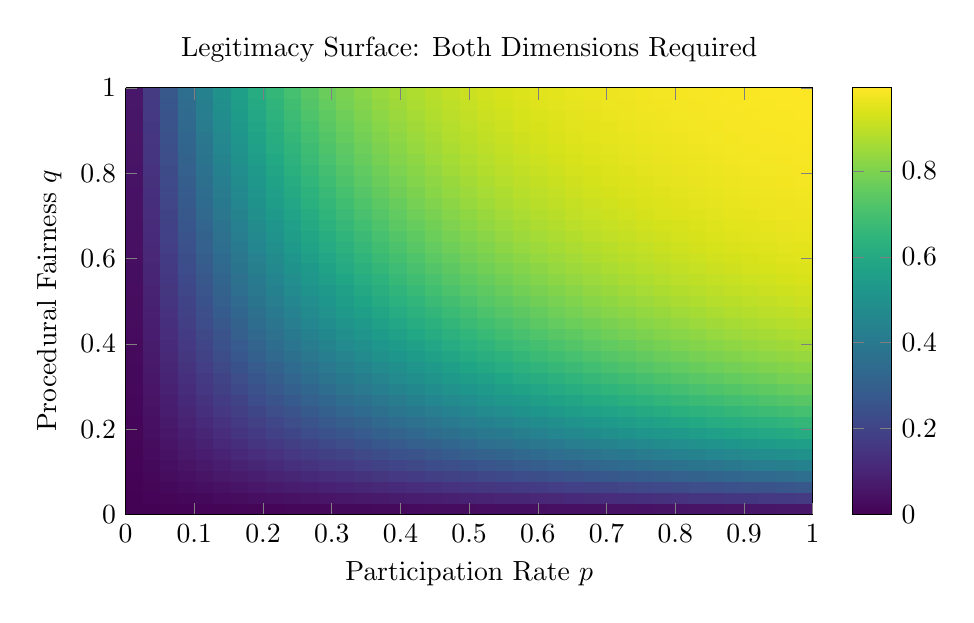
\begin{tikzpicture}
\begin{axis}[
  view={0}{90},
  width=0.85\linewidth, height=7cm,
  xlabel={Participation Rate $p$},
  ylabel={Procedural Fairness $q$},
  colorbar,
  colormap/viridis,
  title={Legitimacy Surface: Both Dimensions Required}
]
\addplot3[
  surf, shader=flat,
  domain=0:1, y domain=0:1,
  samples=40, samples y=40
] {1 - exp(-5*x*y)};
\end{axis}
\end{tikzpicture}
\caption{Legitimacy rises when both participation and procedural fairness are high.}
\end{figure}

\subsubsection{Present Value of a Free Iran}

We cannot price 2,500 years of civilization directly. But we can model the economic value of freedom using present value mathematics.

Let $Y_t$ be annual ``cultural + economic surplus'' attributable to freedom and prosperity, with discount rate $r$:

\begin{equation}
PV = \sum_{t=1}^{T} \frac{Y_t}{(1+r)^t}
\end{equation}

For long-horizon approximation with growth rate $g$ where $r > g$:

\begin{equation}
PV_{\infty} \approx \frac{Y_1}{r - g}
\end{equation}

\textbf{Example}: If a free Iran generates \$100B additional annual surplus over the status quo, with $r = 8\%$ and $g = 3\%$:

\[
PV_{\infty} \approx \frac{\$100B}{0.08 - 0.03} = \$2 \text{ trillion}
\]

This is not speculation---it is the standard approach to valuing long-duration assets.

\subsubsection{Token Value from Captured Share}

For transparency, we present the valuation identity that underlies any rational token pricing:

\begin{equation}
\text{Implied Price} \approx \frac{PV \cdot s \cdot m}{S}
\end{equation}

Where:
\begin{itemize}[leftmargin=*]
    \item $PV$ = Present value of the addressable ``free Iran / diaspora coordination'' economy
    \item $s$ = Capture share (fraction of that economy CYRUS can coordinate)
    \item $m$ = Value accrual fraction (what portion flows to tokenholders via governance, grants, utility)
    \item $S$ = Circulating token supply
\end{itemize}

\begin{figure}[h]
\centering
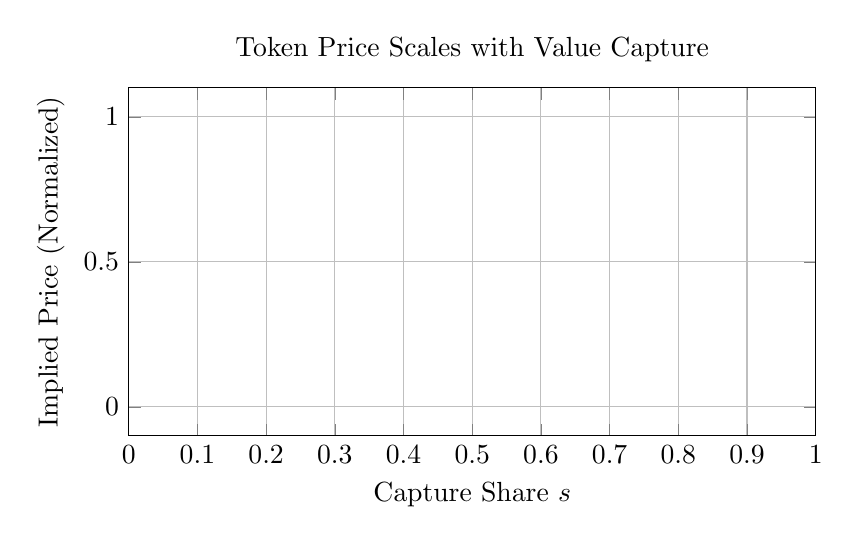
\begin{tikzpicture}
\begin{axis}[
  width=0.85\linewidth, height=6cm,
  xlabel={Capture Share $s$},
  ylabel={Implied Price (Normalized)},
  xmin=0, xmax=0.05,
  grid=both,
  legend pos=north west,
  title={Token Price Scales with Value Capture}
]
\addplot[thick, color=persianblue] {x}; \addlegendentry{$PV \cdot m / S = 1$}
\addplot[thick, color=persiangold] {3*x}; \addlegendentry{$PV \cdot m / S = 3$}
\addplot[thick, color=persianred] {10*x}; \addlegendentry{$PV \cdot m / S = 10$}
\end{axis}
\end{tikzpicture}
\caption{Price scales linearly with capture share; slope depends on value-accrual design.}
\end{figure}

\textbf{Critical Note}: The whitepaper is explicit that $m$ depends on actual mechanisms---governance rights, treasury access, membership utility. Without concrete value accrual, $m \approx 0$ and token value is purely speculative. CYRUS designs for real utility through DAO governance and grant access.

\subsection{How Freedom Wins: The Engineering Summary}

Democracies win sustainably when they:

\begin{enumerate}[leftmargin=*]
    \item \textbf{Reduce the premium on fear}: Rule of law, rights protections, predictable governance make cooperation more attractive than coercion
    \item \textbf{Increase the return to talent}: Education, women's equality, open markets ensure that human capital is developed and deployed efficiently
    \item \textbf{Prevent capture through design}: Checks, transparency, decentralization, and rotation make it structurally difficult for any faction to seize permanent control
\end{enumerate}

This is the engineering lesson of constitutionalism (Montesquieu), legitimacy (Rousseau), and the critique of concentrated power (Marx).

\subsection{The Velvet Path: Nonviolent Transition}

\begin{center}
\textit{``Out beyond ideas of wrongdoing and rightdoing,\\
there is a field. I'll meet you there.\\
When the soul lies down in that grass,\\
the world is too full to talk about.''}\\
\vspace{0.2cm}
--- Rumi
\end{center}

\vspace{0.5cm}

The CYRUS community commits to the \textbf{velvet path}---liberation through legitimacy collapse, not through violence. This is not weakness; it is strategic wisdom rooted in Persian civilization's deepest values.

\subsubsection{Why Nonviolence Wins}

History teaches that violent revolutions often replace one tyranny with another. The French Revolution gave way to the Terror, then Napoleon. The Russian Revolution produced Stalin. The Iranian Revolution of 1979 replaced a flawed monarchy with a theocratic nightmare.

\textbf{Nonviolent transitions, by contrast, build lasting democracies:}
\begin{itemize}[leftmargin=*]
    \item \textbf{Czechoslovakia's Velvet Revolution (1989)}: Peaceful protests, civil disobedience, and moral witness brought down communism without a shot
    \item \textbf{Poland's Solidarity Movement}: Workers, intellectuals, and the Church created parallel institutions that made the regime irrelevant
    \item \textbf{South Africa's Transition}: Despite immense provocation, the ANC chose negotiation and truth-and-reconciliation over vengeance
    \item \textbf{India's Independence}: Gandhi's satyagraha (truth-force) defeated the British Empire through moral authority
\end{itemize}

The pattern is clear: \textit{regimes fall when they lose legitimacy, not when they lose battles.}

\subsubsection{The Persian Way: Cyrus as Model}

Cyrus the Great conquered Babylon without a battle. The gates opened because his reputation preceded him---a reputation for mercy, for honoring local customs, for freeing the enslaved rather than creating new slaves.

\begin{tcolorbox}[colback=persiangold!10!white,colframe=cyruscolor,width=\textwidth,arc=2mm,boxrule=1pt]
\centering
\textbf{Cyrus conquered through legitimacy, not terror.}\\
\vspace{0.2cm}
\textit{The Babylonians welcomed him because he offered something better.\\
This is the model for Iran's liberation: become so obviously better\\
that the regime collapses under the weight of its own illegitimacy.}
\end{tcolorbox}

\subsubsection{How the Diaspora Accelerates Legitimacy Collapse}

The CYRUS DAO contributes to nonviolent regime change by:

\begin{enumerate}[leftmargin=*]
    \item \textbf{Demonstrating Competence}: A well-governed, transparent, effective diaspora institution proves Iranians can self-govern democratically
    \item \textbf{Building Parallel Institutions}: Cultural organizations, educational programs, humanitarian networks that serve Iranians regardless of the regime
    \item \textbf{Documenting Truth}: Funding journalism, human rights documentation, and historical preservation that expose the regime's crimes
    \item \textbf{Maintaining Hope}: Every grant for a Persian language school, every scholarship, every cultural event tells Iranians: \textit{we are building the future}
    \item \textbf{Preparing Transition}: Training administrators, lawyers, educators, and civil servants who will staff a democratic Iran
\end{enumerate}

\textbf{We do not seek to destroy the regime. We seek to make it irrelevant.}

\subsection{Reconciliation, Not Revenge}

\begin{center}
\textit{``If you are irritated by every rub,\\
how will you be polished?''}\\
\vspace{0.2cm}
--- Rumi
\end{center}

\vspace{0.5cm}

When freedom comes---and it \textit{will} come---we face a choice that will define Iran for generations: revenge or reconciliation.

The CYRUS community chooses reconciliation.

\subsubsection{The Poison of Vengeance}

After 1979, the new regime executed thousands. Families were destroyed. Communities were shattered. The cycle of violence that began then continues today---protesters shot, activists hanged, children killed.

If we respond to violence with violence, we perpetuate the cycle. We become what we sought to replace.

\subsubsection{The South African Model}

When apartheid fell, South Africa faced the same choice. Nelson Mandela and Desmond Tutu chose the Truth and Reconciliation Commission---not amnesty without accountability, but a process where perpetrators could confess their crimes in exchange for the truth being heard.

\textbf{Iran will need something similar:}
\begin{itemize}[leftmargin=*]
    \item \textbf{Truth}: Full documentation of crimes---executions, torture, corruption, theft
    \item \textbf{Acknowledgment}: Public recognition of what was done and to whom
    \item \textbf{Accountability}: Those who gave orders face justice; those who followed orders under duress may qualify for amnesty if they confess fully
    \item \textbf{Restitution}: Stolen assets returned; victims' families compensated
    \item \textbf{Healing}: National programs to process collective trauma
\end{itemize}

\subsubsection{Who Is Our Enemy?}

\begin{tcolorbox}[colback=persianblue!10!white,colframe=persianblue,width=\textwidth,arc=3mm,boxrule=2pt]
\centering
\textbf{\Large Our enemy is not the Iranian people who served the regime.}\\
\vspace{0.3cm}
Our enemy is the \textit{system}---the structures of oppression, the mechanisms of control,\\
the ideology that crushes human dignity.\\
\vspace{0.2cm}
Many who work within the system do so to survive, to protect their families,\\
to carve out small spaces of decency within an indecent structure.\\
\vspace{0.2cm}
\textbf{When freedom comes, we will need them to help rebuild.}
\end{tcolorbox}

The revolutionary guards who defect, the bureaucrats who preserve records, the judges who quietly reduce sentences, the teachers who smuggle forbidden ideas into classrooms---these are not our enemies. They are Iranians trapped in an unjust system, waiting for the chance to do better.

\subsubsection{The Example of Reza Pahlavi}

Crown Prince Reza Pahlavi has consistently called for reconciliation rather than revenge. He has:
\begin{itemize}[leftmargin=*]
    \item Refused to demonize ordinary Iranians who work within the system
    \item Called for an inclusive transition that welcomes all Iranians
    \item Emphasized that he seeks no throne---only Iran's freedom
    \item Modeled dignity and restraint despite having every reason for bitterness
\end{itemize}

This is the Cyrus legacy: \textit{mercy to the defeated, welcome to the convert, justice tempered with wisdom.}

\subsection{The Romantic Vision: What a Free Iran Looks Like}

\begin{center}
\textit{``I have lived on the lip of insanity,\\
wanting to know reasons,\\
knocking on a door. It opens.\\
I've been knocking from the inside.''}\\
\vspace{0.2cm}
--- Rumi
\end{center}

\vspace{0.5cm}

Let us paint the picture. Not as fantasy, but as vision---the Iran we are building toward, the Iran that awaits on the other side of this struggle.

\subsubsection{The Return of Persian Culture}

Imagine Tehran in spring. The Alborz mountains still snow-capped, the city blooming with cherry blossoms. But now:

\begin{itemize}[leftmargin=*]
    \item \textbf{Music fills the streets}: The tar and setar, the santur and kamancheh, the voices of singers no longer forbidden. Concerts in Azadi Square. Jazz clubs in Darband. Opera at Vahdat Hall.
    \item \textbf{Women walk freely}: Hair in the wind, faces to the sun. Fashion boutiques on Valiasr. Women CEOs, women judges, women ministers. A woman president, perhaps.
    \item \textbf{Artists create without fear}: Filmmakers telling true stories. Poets publishing without censors. Painters exhibiting without permission. Tehran as the cultural capital of the Middle East once more.
    \item \textbf{Young people dance}: In clubs, at weddings, in the streets during Nowruz. The joy that is every Iranian's birthright, restored.
\end{itemize}

\subsubsection{The Healing of the Land}

Iran's environment has been devastated by mismanagement. A free Iran will:

\begin{itemize}[leftmargin=*]
    \item \textbf{Restore Lake Urmia}: Once the largest lake in the Middle East, now a salt flat. With proper management, it can live again.
    \item \textbf{Replant the forests}: The Hyrcanian forests, older than the ice age, protected and expanded. The Zagros reforested.
    \item \textbf{Clean the air}: Tehran's smog replaced with the clear mountain air that once defined the city.
    \item \textbf{Protect the cheetahs}: The Asiatic cheetah, Iran's national animal, saved from extinction. Persian fallow deer roaming free.
\end{itemize}

\subsubsection{The Return of the Diaspora}

Eight million Iranians live abroad. Many dream of return. A free Iran means:

\begin{itemize}[leftmargin=*]
    \item \textbf{Grandchildren meeting grandparents}: Families reunited after decades of separation
    \item \textbf{Skills coming home}: Engineers, doctors, scientists, entrepreneurs bringing expertise built abroad
    \item \textbf{Investment flowing in}: Diaspora capital rebuilding infrastructure, starting businesses, creating jobs
    \item \textbf{Dual lives}: Some will return permanently. Others will split time. All will finally have the \textit{choice}.
\end{itemize}

\subsubsection{Iran Among Nations}

A free, democratic Iran transforms the region:

\begin{itemize}[leftmargin=*]
    \item \textbf{Peace with neighbors}: No more funding of proxy wars. Normal relations with Arab states, Israel, the West.
    \item \textbf{Economic integration}: Iran's oil and gas, but also tech, tourism, agriculture. The Silk Road reborn.
    \item \textbf{Cultural leadership}: Persian language, art, and philosophy inspiring the world as they did for millennia.
    \item \textbf{Moral authority}: A nation that freed itself nonviolently, reconciled with its past, and built a just future. A model for others.
\end{itemize}

\subsection{A Love Letter to Iran}

\begin{center}
\textit{``Let the beauty we love be what we do.\\
There are hundreds of ways to kneel and kiss the ground.''}\\
\vspace{0.2cm}
--- Rumi
\end{center}

\vspace{0.5cm}

To Iran---

You are not the regime that occupies you.

You are the mountains and the deserts, the Caspian shores and the Persian Gulf. You are Persepolis and Pasargadae, Isfahan and Shiraz. You are the poetry of Hafez and Rumi, the mathematics of Khayyam, the medicine of Avicenna.

You are the grandmother who still makes tahdig perfectly. The grandfather who recites Shahnameh from memory. The mother who teaches her daughter to read despite the morality police. The father who dreams of a better future for his sons.

You are the young woman who removed her hijab and walked into history. The student who tweeted and went to prison. The worker who struck. The artist who painted forbidden dreams. The musician who played forbidden songs.

You are 85 million people carrying 2,500 years of civilization in your hearts.

\textbf{You are not defeated. You are not forgotten. You are not alone.}

We, your children scattered across the earth, hold you in our hearts. We build this token, this DAO, this movement---not for profit, not for power---but for \textit{you}.

Every CYRUS token is a vote for your freedom.\\
Every proposal passed is a brick in your future.\\
Every grant given is a seed planted in your soil.

We will not rest until you are free.

We will not rest until your daughters walk in sunlight.\\
Until your sons sing without fear.\\
Until your poets write without censors.\\
Until your scientists discover without limits.\\
Until your lovers love without hiding.

\textit{M\=a ham\=e b\=a ham hast\=im.}\\
We are all together.

\textit{Zendeh b\=ad Ir\=an.}\\
Long live Iran.

\begin{tcolorbox}[colback=persiangold!10!white,colframe=persianblue,width=\textwidth,arc=3mm,boxrule=2pt]
\centering
\textbf{\Large The CYRUS Thesis}

\vspace{0.3cm}

A transparent, decentralized, constitutionally constrained DAO---\\
governed by the Persian diaspora, funded by the bonding curve,\\
and oriented toward liberation and reconstruction---\\
is a \textit{structurally superior} institution for achieving freedom\\
compared to any centralized alternative.

\vspace{0.3cm}

\textit{This is not hope. This is design.}
\end{tcolorbox}
